\documentclass[border=1pt]{standalone}
\usepackage[T1]{fontenc}
\usepackage{times}
\usepackage{amsmath,amssymb}
\usepackage{tikz}
\usetikzlibrary{arrows.meta,calc,decorations.pathreplacing}
\definecolor{ink}{HTML}{222222}
\definecolor{muted}{HTML}{767676}
\definecolor{ours}{HTML}{1f5fa8}
\definecolor{oursbg}{HTML}{eef3fa}
\definecolor{boxbg}{HTML}{f7f7f5}
\definecolor{cA}{HTML}{2a9d8f}
\definecolor{cB}{HTML}{c8641c}
\definecolor{cC}{HTML}{7b5ea7}
\begin{document}
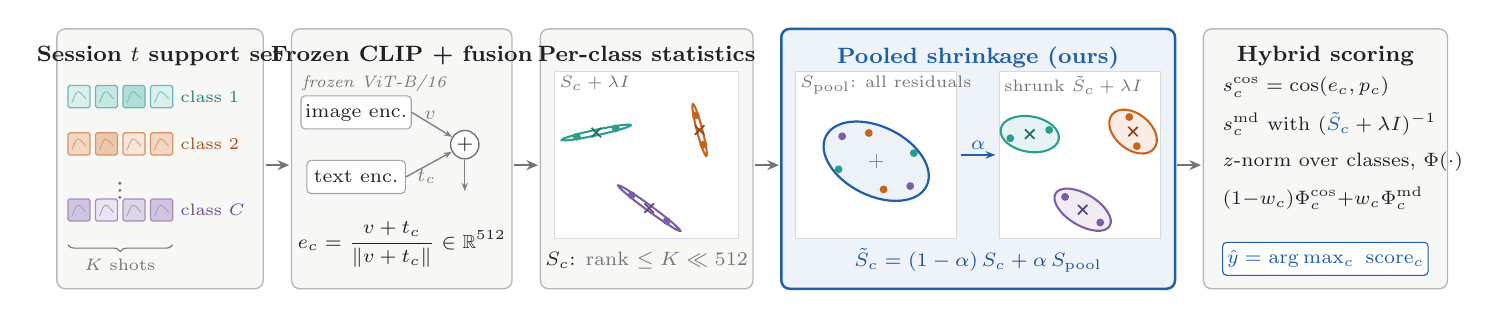
\begin{tikzpicture}[font=\fontsize{7.2}{8.4}\selectfont, ink,
  box/.style={rounded corners=3pt, draw=black!28, fill=boxbg, line width=0.5pt},
  oursbox/.style={rounded corners=3pt, draw=ours, fill=oursbg, line width=0.9pt},
  title/.style={font=\fontsize{7.6}{9}\selectfont\bfseries, anchor=north},
  flow/.style={-{Stealth[length=4.2pt,width=3.6pt]}, line width=0.8pt, black!55},
  chip/.style={rounded corners=1.5pt, draw=black!35, fill=white, line width=0.4pt, minimum height=0.42cm, inner sep=1.5pt},
  panelframe/.style={draw=black!15, line width=0.3pt, fill=white},
  tag/.style={anchor=north west, font=\fontsize{5.9}{6.6}\selectfont, text=muted, inner sep=1.6pt}]
\path[box] (0.00,0) rectangle (2.62,3.3);
\path[box] (2.98,0) rectangle (5.78,3.3);
\path[box] (6.14,0) rectangle (8.84,3.3);
\path[oursbox] (9.20,0) rectangle (14.20,3.3);
\path[box] (14.56,0) rectangle (17.66,3.3);
\node[title] at (1.31,3.1999999999999997) {Session $t$ support set};
\node[title] at (4.38,3.1999999999999997) {Frozen CLIP + fusion};
\node[title] at (7.49,3.1999999999999997) {Per-class statistics};
\node[title, text=ours] at (11.70,3.1999999999999997) {Pooled shrinkage (ours)};
\node[title] at (16.11,3.1999999999999997) {Hybrid scoring};
\draw[flow] (2.65,1.57) -- (2.95,1.57);
\draw[flow] (5.81,1.57) -- (6.11,1.57);
\draw[flow] (8.87,1.57) -- (9.17,1.57);
\draw[flow] (14.23,1.57) -- (14.53,1.57);
\path[fill=cA!16, draw=cA!70, line width=0.45pt, rounded corners=0.6pt] (0.14,2.30) rectangle ++(0.28,0.28);
\draw[cA!60, line width=0.35pt] (0.19,2.36) .. controls (0.26,2.54) .. (0.37,2.41);
\path[fill=cA!26, draw=cA!70, line width=0.45pt, rounded corners=0.6pt] (0.49,2.30) rectangle ++(0.28,0.28);
\draw[cA!60, line width=0.35pt] (0.54,2.36) .. controls (0.61,2.54) .. (0.72,2.41);
\path[fill=cA!36, draw=cA!70, line width=0.45pt, rounded corners=0.6pt] (0.84,2.30) rectangle ++(0.28,0.28);
\draw[cA!60, line width=0.35pt] (0.89,2.36) .. controls (0.96,2.54) .. (1.07,2.41);
\path[fill=cA!16, draw=cA!70, line width=0.45pt, rounded corners=0.6pt] (1.19,2.30) rectangle ++(0.28,0.28);
\draw[cA!60, line width=0.35pt] (1.24,2.36) .. controls (1.31,2.54) .. (1.42,2.41);
\node[anchor=west, font=\fontsize{6.3}{7.4}\selectfont, text=cA!80!black, inner sep=1pt] at (1.53,2.44) {class 1};
\path[fill=cB!26, draw=cB!70, line width=0.45pt, rounded corners=0.6pt] (0.14,1.70) rectangle ++(0.28,0.28);
\draw[cB!60, line width=0.35pt] (0.19,1.76) .. controls (0.26,1.94) .. (0.37,1.81);
\path[fill=cB!36, draw=cB!70, line width=0.45pt, rounded corners=0.6pt] (0.49,1.70) rectangle ++(0.28,0.28);
\draw[cB!60, line width=0.35pt] (0.54,1.76) .. controls (0.61,1.94) .. (0.72,1.81);
\path[fill=cB!16, draw=cB!70, line width=0.45pt, rounded corners=0.6pt] (0.84,1.70) rectangle ++(0.28,0.28);
\draw[cB!60, line width=0.35pt] (0.89,1.76) .. controls (0.96,1.94) .. (1.07,1.81);
\path[fill=cB!26, draw=cB!70, line width=0.45pt, rounded corners=0.6pt] (1.19,1.70) rectangle ++(0.28,0.28);
\draw[cB!60, line width=0.35pt] (1.24,1.76) .. controls (1.31,1.94) .. (1.42,1.81);
\node[anchor=west, font=\fontsize{6.3}{7.4}\selectfont, text=cB!80!black, inner sep=1pt] at (1.53,1.84) {class 2};
\path[fill=cC!36, draw=cC!70, line width=0.45pt, rounded corners=0.6pt] (0.14,0.86) rectangle ++(0.28,0.28);
\draw[cC!60, line width=0.35pt] (0.19,0.92) .. controls (0.26,1.10) .. (0.37,0.97);
\path[fill=cC!16, draw=cC!70, line width=0.45pt, rounded corners=0.6pt] (0.49,0.86) rectangle ++(0.28,0.28);
\draw[cC!60, line width=0.35pt] (0.54,0.92) .. controls (0.61,1.10) .. (0.72,0.97);
\path[fill=cC!26, draw=cC!70, line width=0.45pt, rounded corners=0.6pt] (0.84,0.86) rectangle ++(0.28,0.28);
\draw[cC!60, line width=0.35pt] (0.89,0.92) .. controls (0.96,1.10) .. (1.07,0.97);
\path[fill=cC!36, draw=cC!70, line width=0.45pt, rounded corners=0.6pt] (1.19,0.86) rectangle ++(0.28,0.28);
\draw[cC!60, line width=0.35pt] (1.24,0.92) .. controls (1.31,1.10) .. (1.42,0.97);
\node[anchor=west, font=\fontsize{6.3}{7.4}\selectfont, text=cC!80!black, inner sep=1pt] at (1.53,1.00) {class $C$};
\fill[muted] (0.80,1.16) circle (0.021);
\fill[muted] (0.80,1.25) circle (0.021);
\fill[muted] (0.80,1.34) circle (0.021);
\draw[decorate, decoration={brace, amplitude=2.5pt, mirror}, muted, line width=0.4pt] (0.14,0.56) -- (1.47,0.56);
\node[text=muted, font=\fontsize{6.5}{7.6}\selectfont] at (0.80,0.30) {$K$ shots};
\node[chip, minimum width=1.25cm] (ie) at (3.80,2.24) {image enc.};
\node[chip, minimum width=1.25cm] (te) at (3.80,1.42) {text enc.};
\node[font=\fontsize{6}{7.1}\selectfont, text=muted, anchor=south west, inner sep=0.5pt] at ($(ie.north west)+(0,0.02)$) {\itshape frozen ViT-B/16};
\node[draw=black!55, circle, inner sep=0.2pt, minimum size=0.36cm, fill=white, line width=0.5pt] (plus) at (5.18,1.83) {$+$};
\draw[-{Stealth[length=3pt]}, black!50, line width=0.5pt] (ie.east) -- node[above, pos=0.45, inner sep=1pt] {$v$} (plus);
\draw[-{Stealth[length=3pt]}, black!50, line width=0.5pt] (te.east) -- node[below, pos=0.45, inner sep=1pt] {$t_c$} (plus);
\draw[-{Stealth[length=3pt]}, black!50, line width=0.5pt] (plus.south) -- ++(0,-0.40);
\node[font=\fontsize{6.8}{7.9}\selectfont] at (4.38,0.56) {$e_c=\dfrac{v+t_c}{\lVert v+t_c\rVert}\in\mathbb{R}^{512}$};
\path[panelframe] (6.32,0.64) rectangle (8.66,2.76);
\node[tag] at (6.32,2.76) {$S_c+\lambda I$};
\draw[cA, line width=0.75pt] (6.850,1.984) ellipse[x radius=0.448, y radius=0.035, rotate=-167.8];
\fill[cA] (7.097,2.037) circle (0.05);
\fill[cA] (6.603,1.931) circle (0.05);
\draw[cA!70!black, line width=0.6pt] (6.790,1.924) -- (6.910,2.044) (6.790,2.044) -- (6.910,1.924);
\draw[cB, line width=0.75pt] (8.162,2.016) ellipse[x radius=0.340, y radius=0.035, rotate=104.6];
\fill[cB] (8.114,2.201) circle (0.05);
\fill[cB] (8.210,1.831) circle (0.05);
\draw[cB!70!black, line width=0.6pt] (8.102,1.956) -- (8.222,2.076) (8.102,2.076) -- (8.222,1.956);
\draw[cC, line width=0.75pt] (7.522,1.024) ellipse[x radius=0.490, y radius=0.035, rotate=143.8];
\fill[cC] (7.745,0.861) circle (0.05);
\fill[cC] (7.299,1.187) circle (0.05);
\draw[cC!70!black, line width=0.6pt] (7.462,0.964) -- (7.582,1.084) (7.462,1.084) -- (7.582,0.964);
\node[font=\fontsize{6.6}{7.7}\selectfont] at (7.49,0.36) {$S_c$: \textcolor{muted}{rank $\le K\ll 512$}};
\path[panelframe] (9.38,0.64) rectangle (11.43,2.76);
\path[panelframe] (11.97,0.64) rectangle (14.02,2.76);
\node[tag] at (9.38,2.76) {$S_{\mathrm{pool}}$: all residuals};
\node[tag] at (11.97,2.76) {shrunk $\tilde S_c+\lambda I$};
\draw[ours, line width=0.8pt, fill=ours!8] (10.405,1.620) ellipse[x radius=0.713, y radius=0.438, rotate=153.7];
\draw[black!45, line width=0.35pt] (10.315,1.620) -- (10.495,1.620) (10.405,1.530) -- (10.405,1.710);
\fill[cA] (10.883,1.723) circle (0.05);
\fill[cA] (9.927,1.517) circle (0.05);
\fill[cB] (10.311,1.978) circle (0.05);
\fill[cB] (10.499,1.262) circle (0.05);
\fill[cC] (10.837,1.304) circle (0.05);
\fill[cC] (9.973,1.936) circle (0.05);
\draw[cA, line width=0.75pt, fill=cA!12] (12.355,1.964) ellipse[x radius=0.374, y radius=0.225, rotate=170.2];
\fill[cA] (12.602,2.017) circle (0.05);
\fill[cA] (12.108,1.911) circle (0.05);
\draw[cA!70!black, line width=0.6pt] (12.295,1.904) -- (12.415,2.024) (12.295,2.024) -- (12.415,1.904);
\draw[cB, line width=0.75pt, fill=cB!12] (13.667,1.996) ellipse[x radius=0.343, y radius=0.227, rotate=140.9];
\fill[cB] (13.619,2.181) circle (0.05);
\fill[cB] (13.715,1.811) circle (0.05);
\draw[cB!70!black, line width=0.6pt] (13.607,1.936) -- (13.727,2.056) (13.607,2.056) -- (13.727,1.936);
\draw[cC, line width=0.75pt, fill=cC!12] (13.027,1.004) ellipse[x radius=0.401, y radius=0.199, rotate=148.9];
\fill[cC] (13.250,0.841) circle (0.05);
\fill[cC] (12.804,1.167) circle (0.05);
\draw[cC!70!black, line width=0.6pt] (12.967,0.944) -- (13.087,1.064) (12.967,1.064) -- (13.087,0.944);
\draw[-{Stealth[length=3.6pt]}, ours, line width=0.8pt] (11.48,1.70) -- node[above, inner sep=1.5pt, font=\fontsize{6.8}{7.9}\selectfont] {$\alpha$} (11.92,1.70);
\node[font=\fontsize{6.8}{7.9}\selectfont, text=ours!85!black] at (11.70,0.36) {$\tilde S_c=(1-\alpha)\,S_c+\alpha\,S_{\mathrm{pool}}$};
\node[anchor=west, font=\fontsize{6.7}{7.8}\selectfont] at (14.68,2.56) {$s^{\cos}_c=\cos(e_c,p_c)$};
\node[anchor=west, font=\fontsize{6.7}{7.8}\selectfont] at (14.68,2.09) {$s^{\mathrm{md}}_c$ with $(\textcolor{ours}{\tilde S_c}+\lambda I)^{-1}$};
\node[anchor=west, font=\fontsize{6.7}{7.8}\selectfont] at (14.68,1.62) {$z$-norm over classes, $\Phi(\cdot)$};
\node[anchor=west, font=\fontsize{6.7}{7.8}\selectfont] at (14.68,1.15) {$(1{-}w_c)\Phi^{\cos}_c{+}w_c\Phi^{\mathrm{md}}_c$};
\node[chip, draw=ours, text=ours, font=\fontsize{6.8}{7.9}\selectfont, minimum width=2.3cm] at (16.11,0.38) {$\hat y=\arg\max_c\ \mathrm{score}_c$};
\end{tikzpicture}
\end{document}